\section{User Manual}

\subsection{Sign in}
\begin{figure}[H]
	\centering
	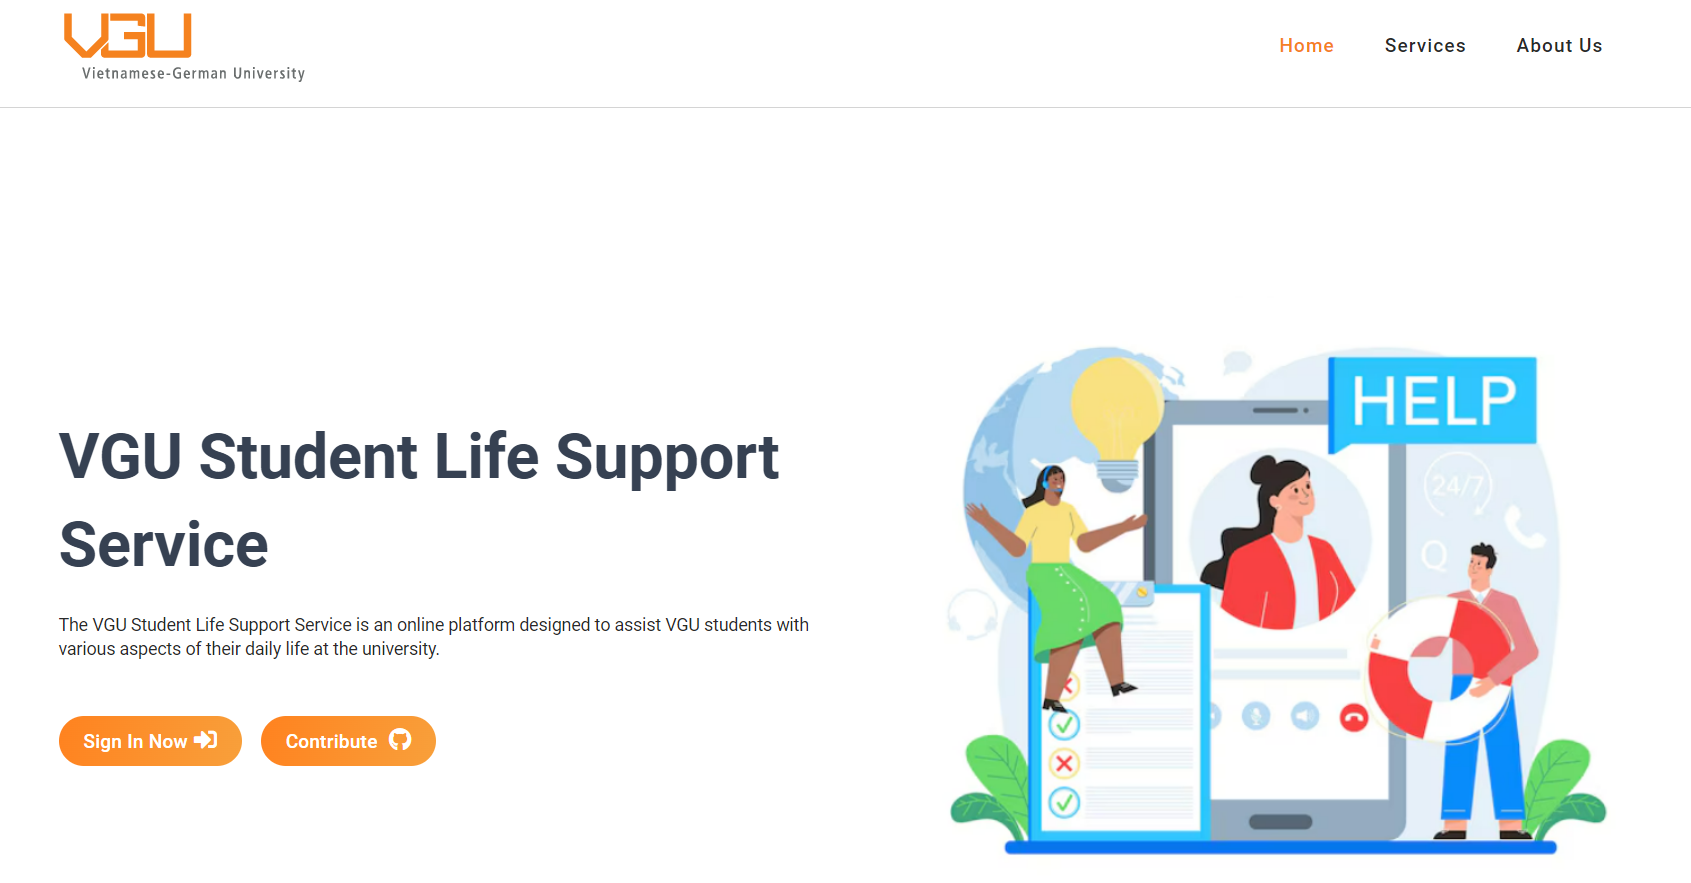
\includegraphics[width=1.\linewidth]{graphics/gui/user/landing}
	\caption{Landing Page}
	\label{fig:landing}
\end{figure}

In the landing page of the service, navigate to Login page by clicking "Sign In Now"


\begin{figure}[H]
	\centering
	\begin{minipage}{.5\textwidth}
		\centering
		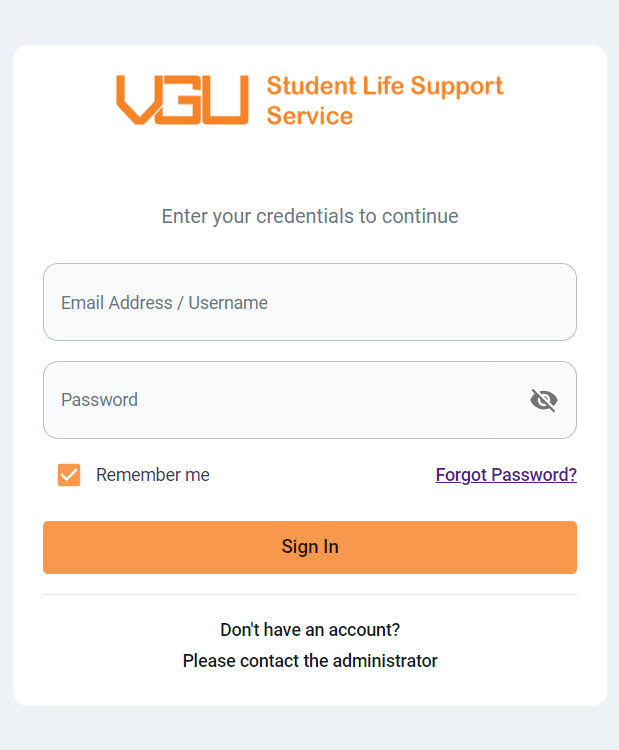
\includegraphics[width=.9\linewidth]{graphics/gui/user/login.png}
		\captionof{figure}{Sign in Form}
		\label{fig:gui-login}
	\end{minipage}%
	\begin{minipage}{.5\textwidth}
		\centering
		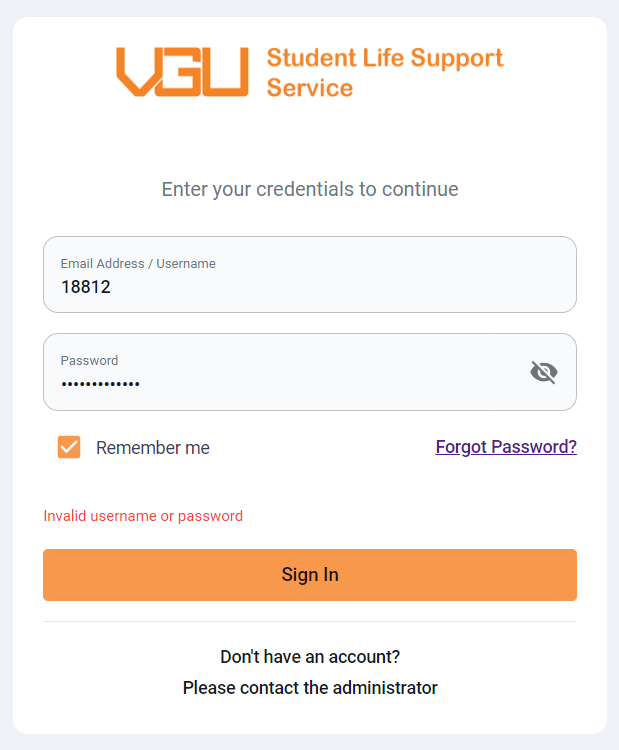
\includegraphics[width=0.9\linewidth]{graphics/gui/user/login-error.png}
		\captionof{figure}{Failed Sign in attempt}
		\label{fig:gui-login-failed}
	\end{minipage}
\end{figure}



To access the service, input your username (or email) and password, then click on the sign-in button (refer to Figure \ref{fig:gui-login}). If you provide incorrect credentials, a warning message will appear, indicating that you need to correct either your username or password (Figure \ref{fig:gui-login-failed}).





\subsection{Forgot password}

%In case of forgetting your password, you can reset it by clicking 'Forgot Password?' of the 'Sign in' form (see Firgure \ref{fig:gui-login}). Then, enter your the email in the 'Forgot Password' form adn click 'Reset Password' (Figure \ref{fig:gui-forgot-pass})

If you forget your password, you can initiate a reset by selecting the 'Forgot Password?' option on the 'Sign in' form (refer to Figure \ref{fig:gui-login}). Subsequently, provide your email address in the 'Forgot Password' form and click on 'Reset Password' (see Figure \ref{fig:gui-forgot-pass}).

\begin{figure}[H]
	\centering
	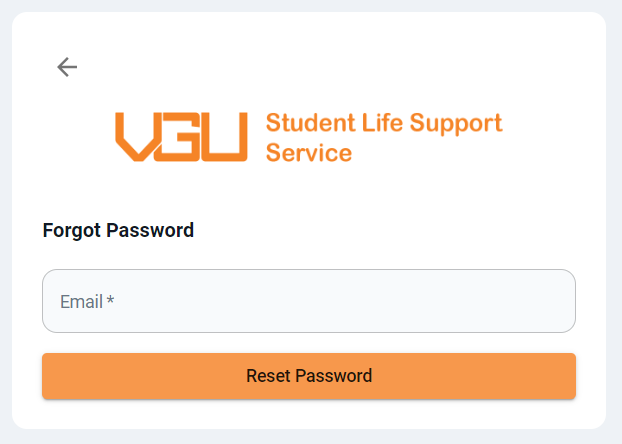
\includegraphics[width=0.7\linewidth]{graphics/gui/user/reset-pass.png}
	\caption{Reset Password Form}
	\label{fig:gui-forgot-pass}
\end{figure}



If your email is associated with an account in the system, a success notification will appear, and password reset instructions will be sent to your email (Figure \ref{fig:gui-reset-pass-success}, \ref{fig:gui-email-reset-pass}).  Conversely, if the email is not found in the system, a failure notification will indicate that the email does not exist (Figure \ref{fig:gui-reset-pass-failed}).

\begin{figure}[H]
	\centering
	\begin{minipage}{.5\textwidth}
		\centering
		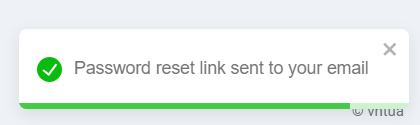
\includegraphics[width=.9\linewidth]{graphics/gui/user/reset-pass-success.png}
		\captionof{figure}{Reset password successfully}
		\label{fig:gui-reset-pass-success}
	\end{minipage}%
	\begin{minipage}{.5\textwidth}
		\centering
		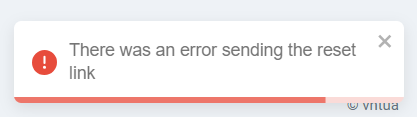
\includegraphics[width=0.9\linewidth]{graphics/gui/user/reset-pass-failed.png}
		\captionof{figure}{Reset password failed}
		\label{fig:gui-reset-pass-failed}
	\end{minipage}
\end{figure}


\begin{figure}[H]
	\centering
	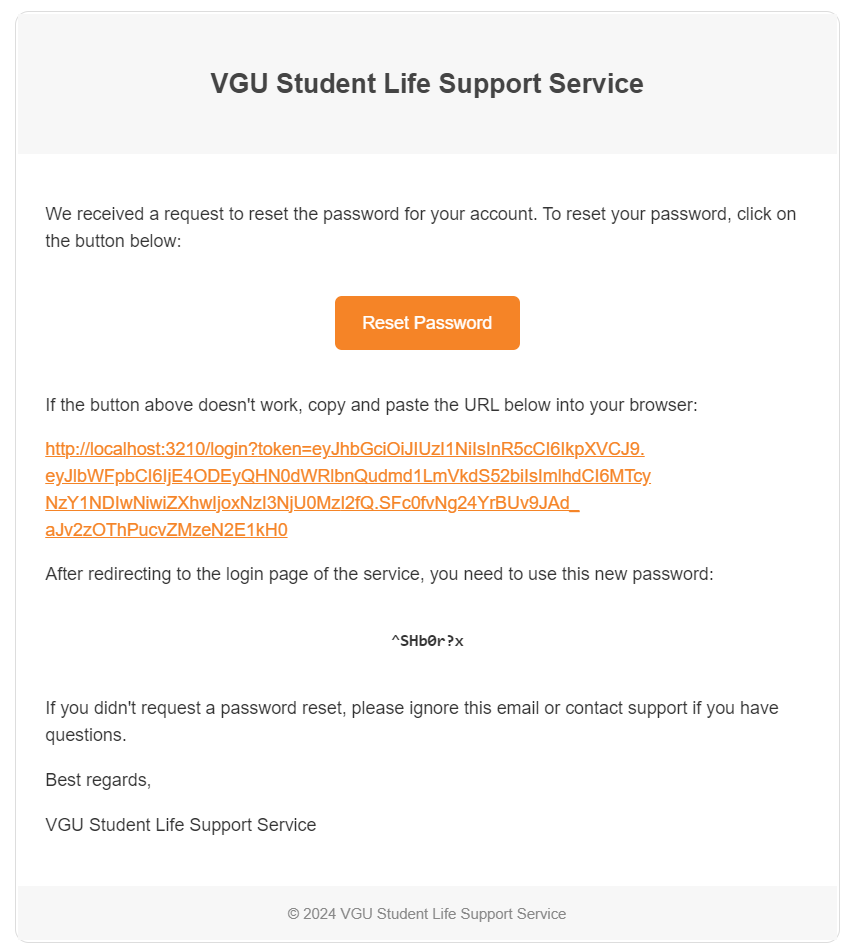
\includegraphics[width=0.8\linewidth]{graphics/gui/user/email-reset.png}
	\caption{Reset password email instructions}
	\label{fig:gui-email-reset-pass}
\end{figure}


\subsection{Student's functions}
After logging in successfully, you will be navigated to the homepage

\begin{figure}[H]
	\centering
	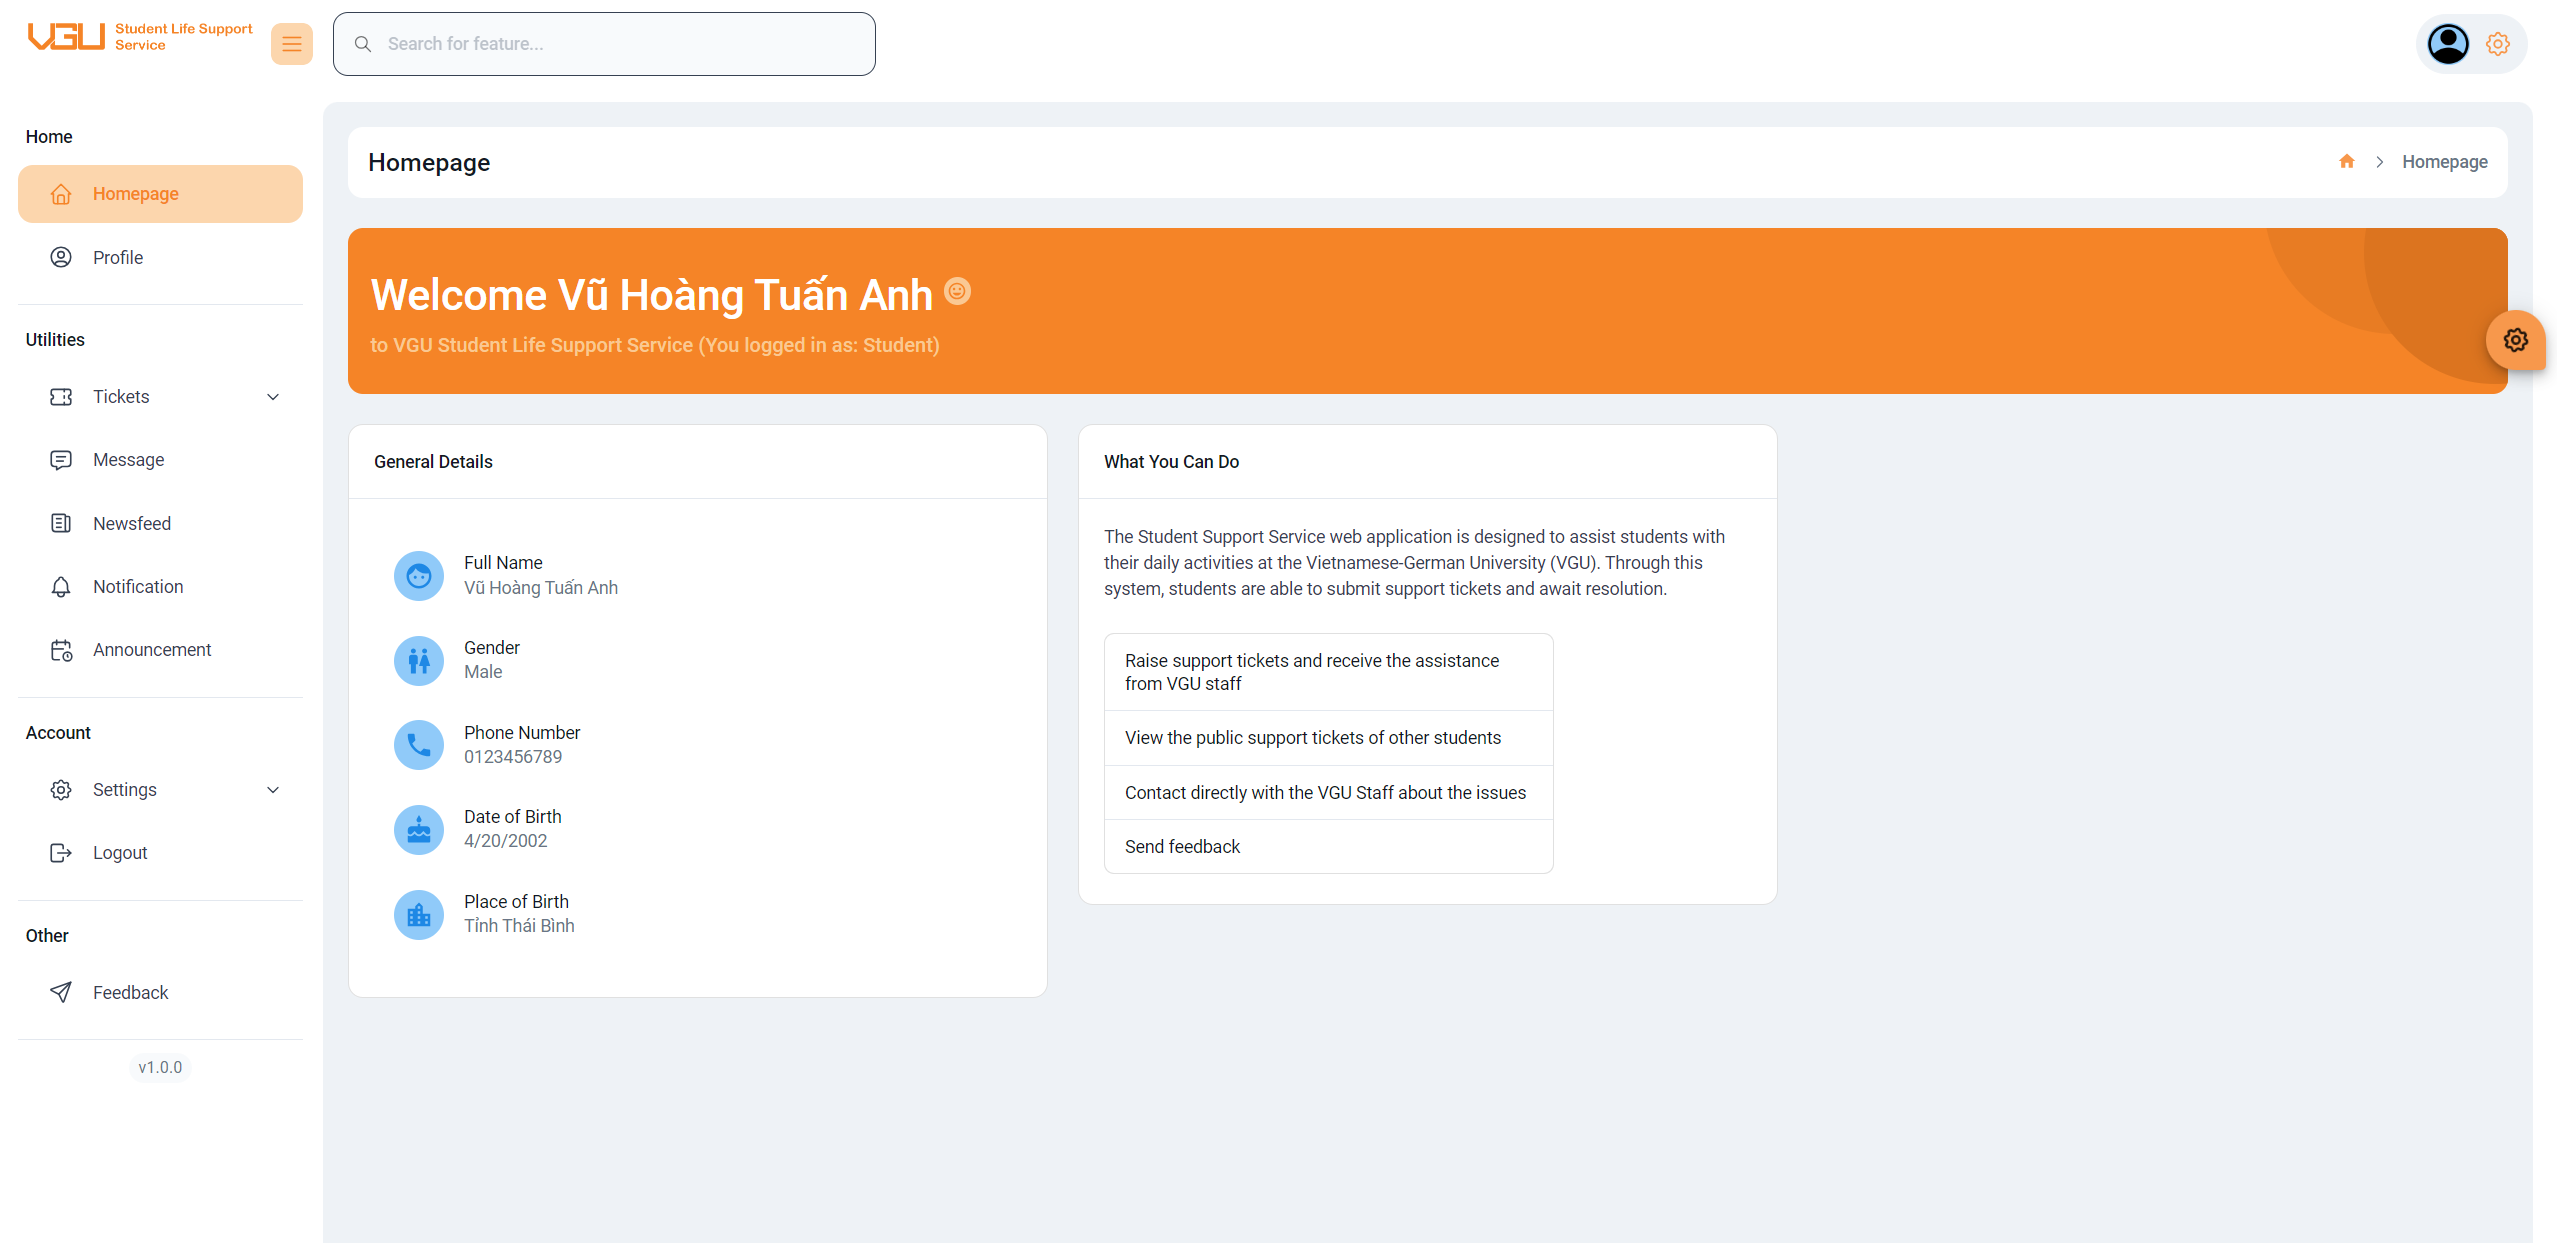
\includegraphics[width=1.0\linewidth]{graphics/gui/student/homepage}
	\caption{Student's Home Page}
	\label{fig:gui-std-homepage}
\end{figure}


	\subsubsection{View Profile}
	\begin{figure}[H]
		\centering
		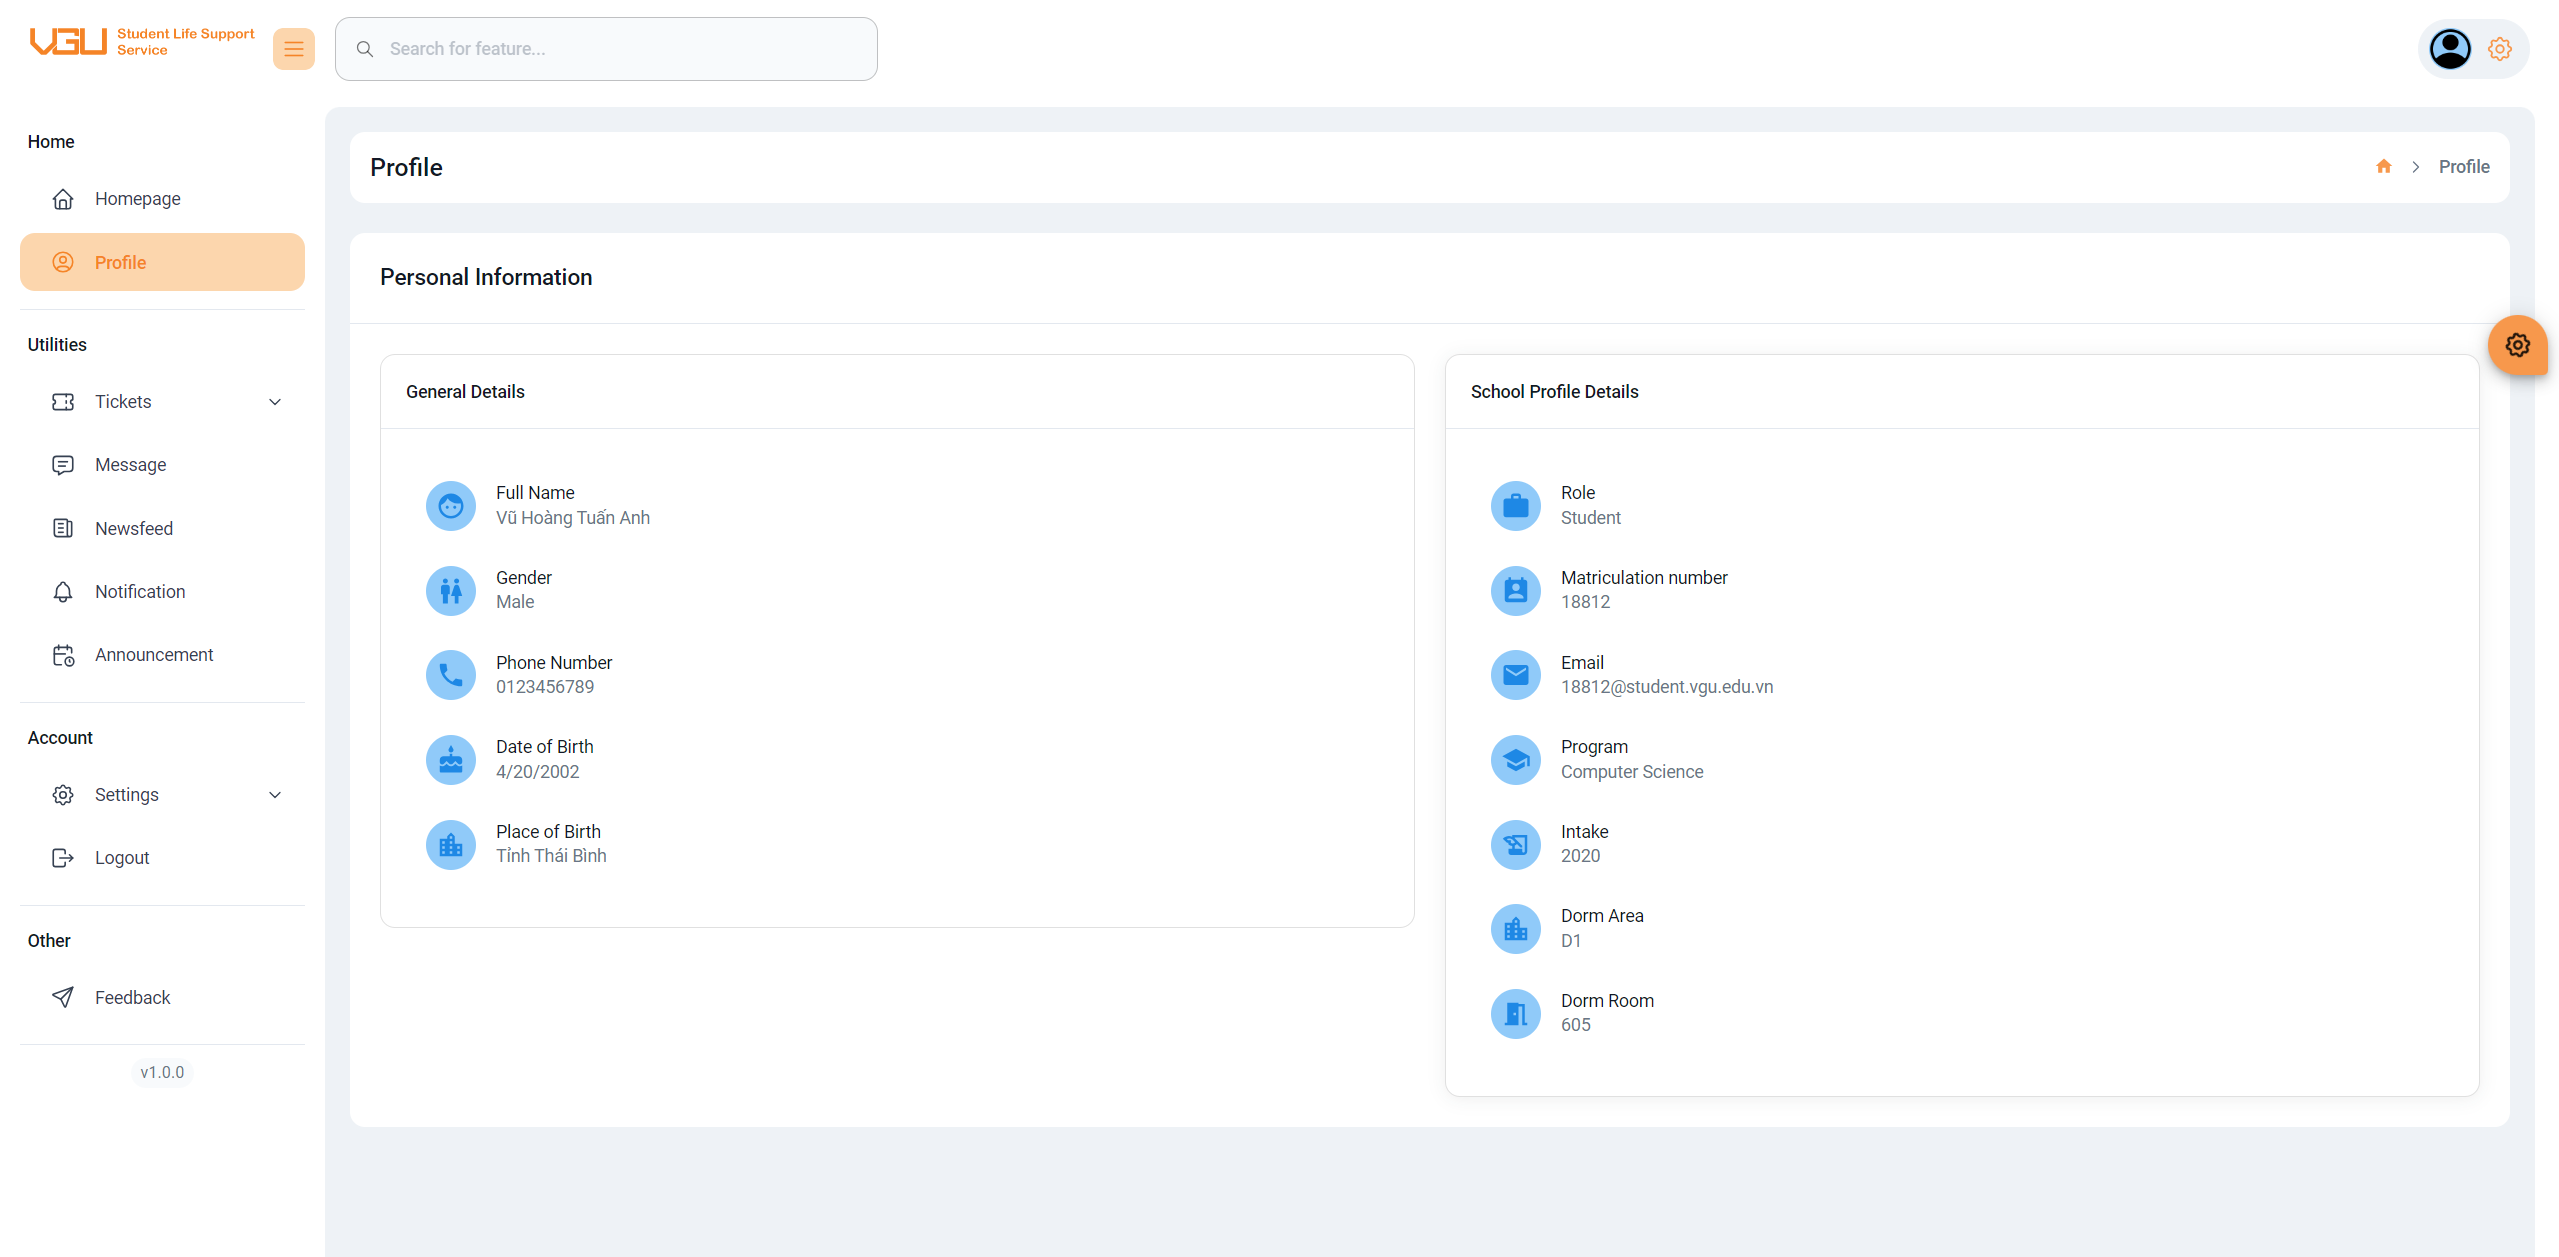
\includegraphics[width=1.0\linewidth]{graphics/gui/student/profile}
		\caption{Student's Profile Page}
		\label{fig:gui-std-profile}
	\end{figure}
	
	
	\subsubsection{View Tickets}
	\begin{figure}[H]
		\centering
		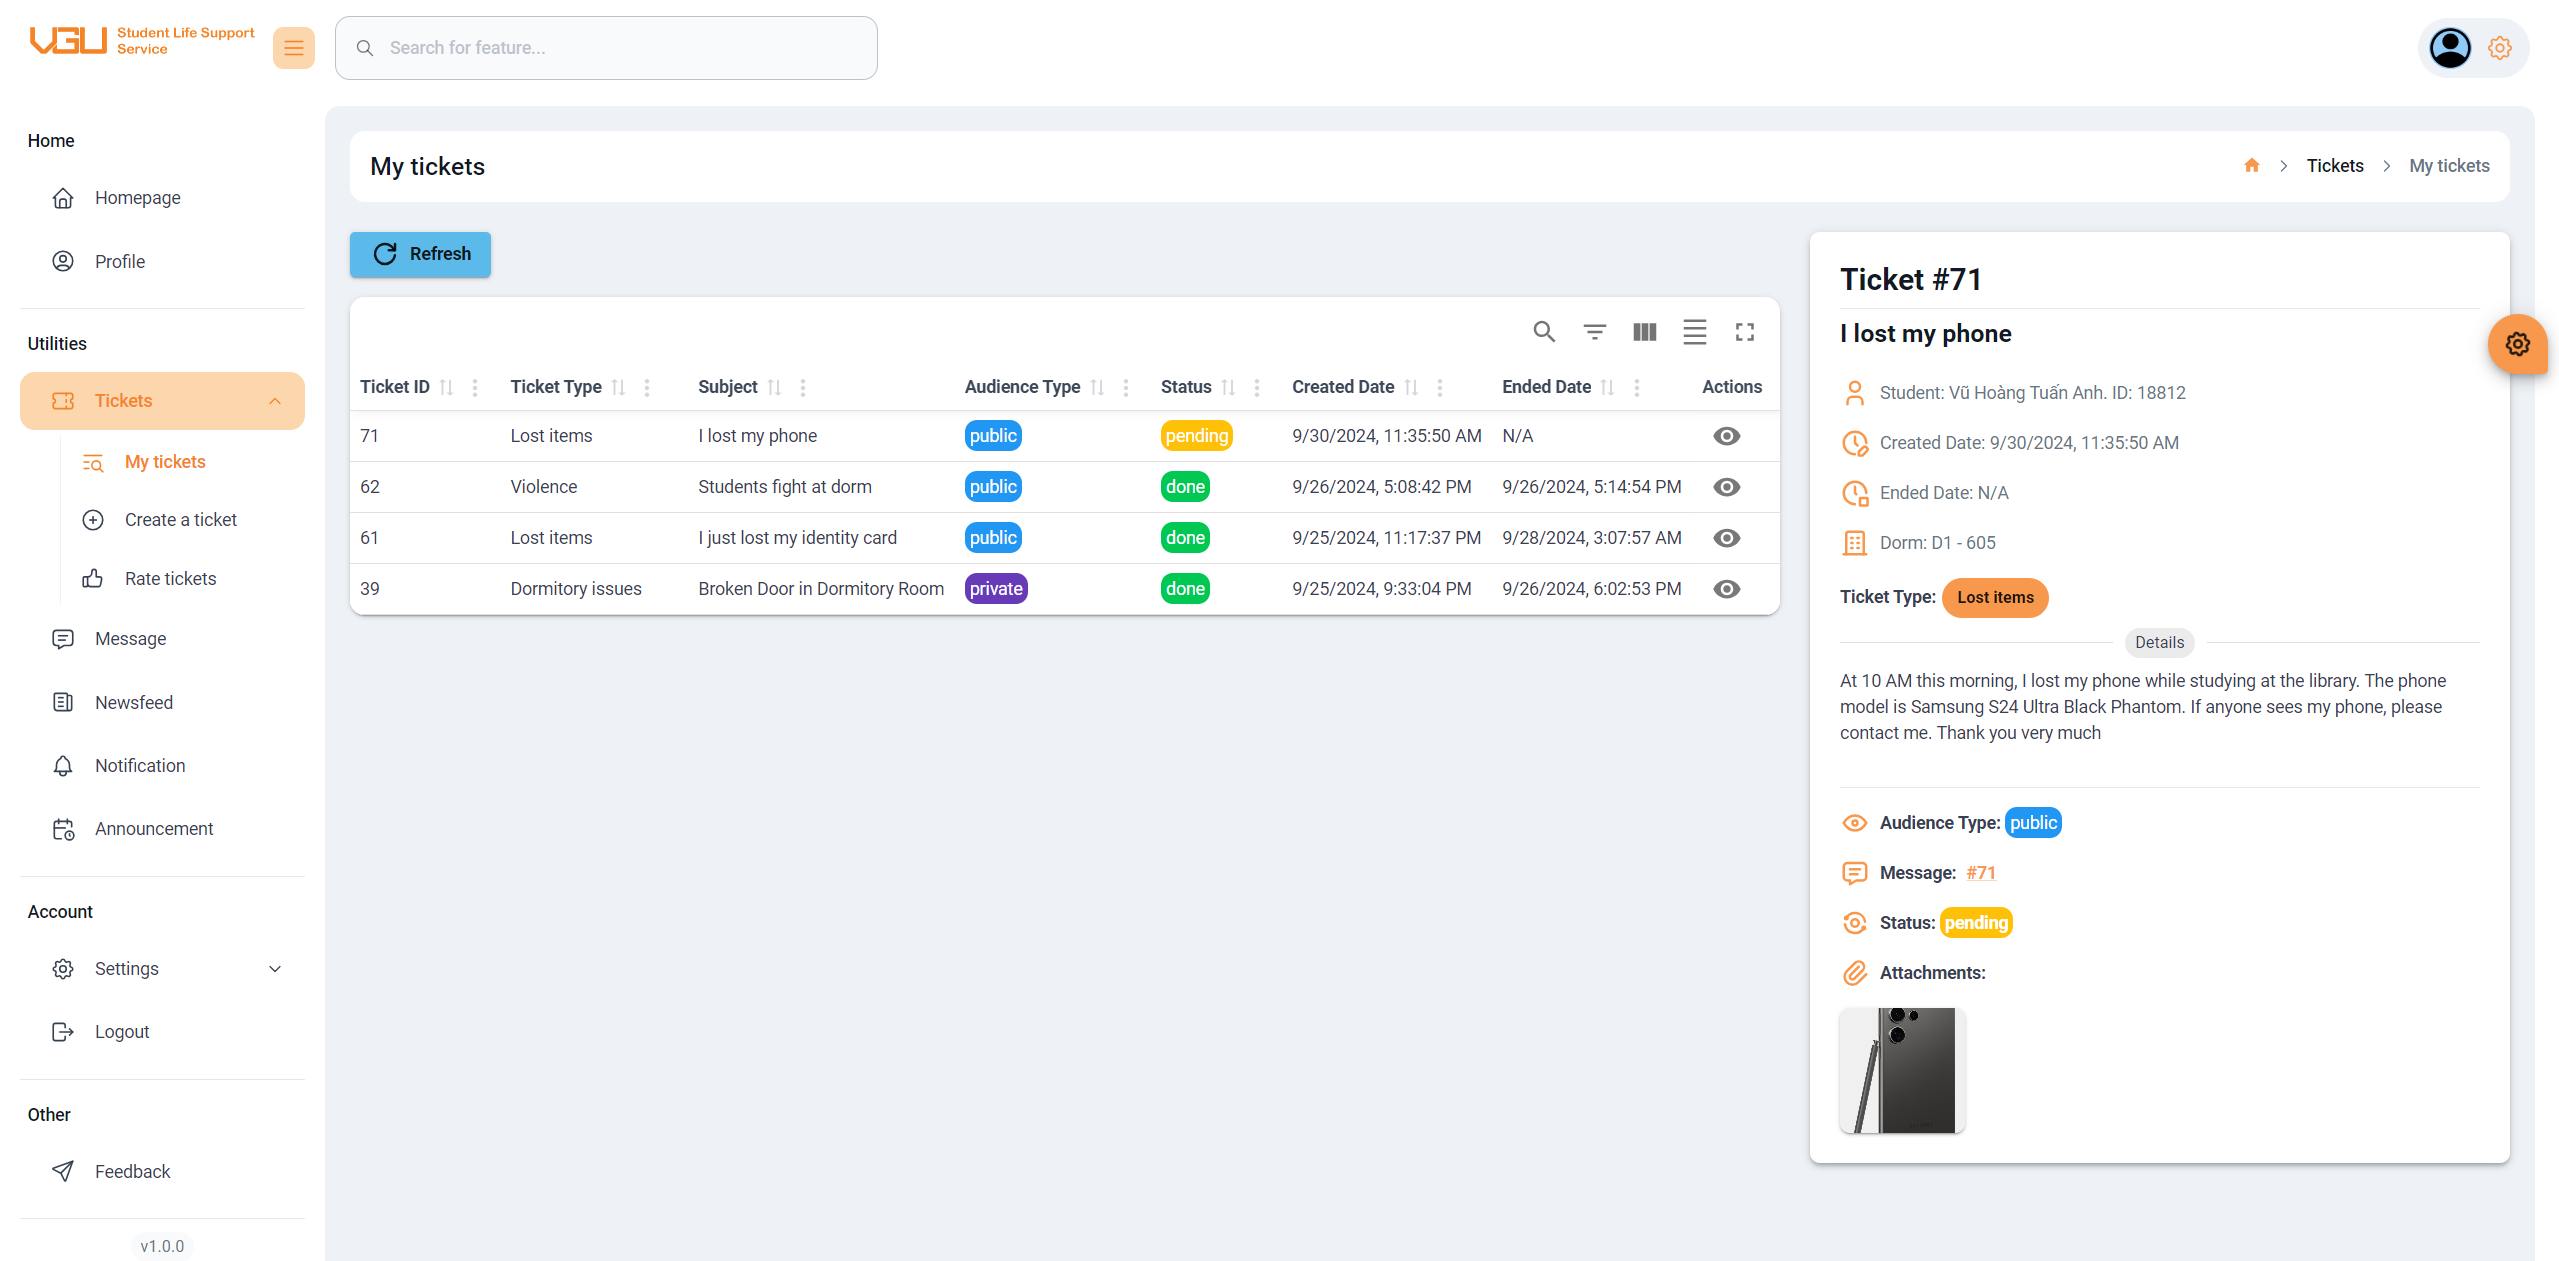
\includegraphics[width=1.0\linewidth]{graphics/gui/student/my-tickets}
		\caption{Student's Tickets List Page}
		\label{fig:gui-std-my-tickets}
	\end{figure}
	
	
	\subsubsection{Create Tickets}
	\begin{figure}[H]
		\centering
		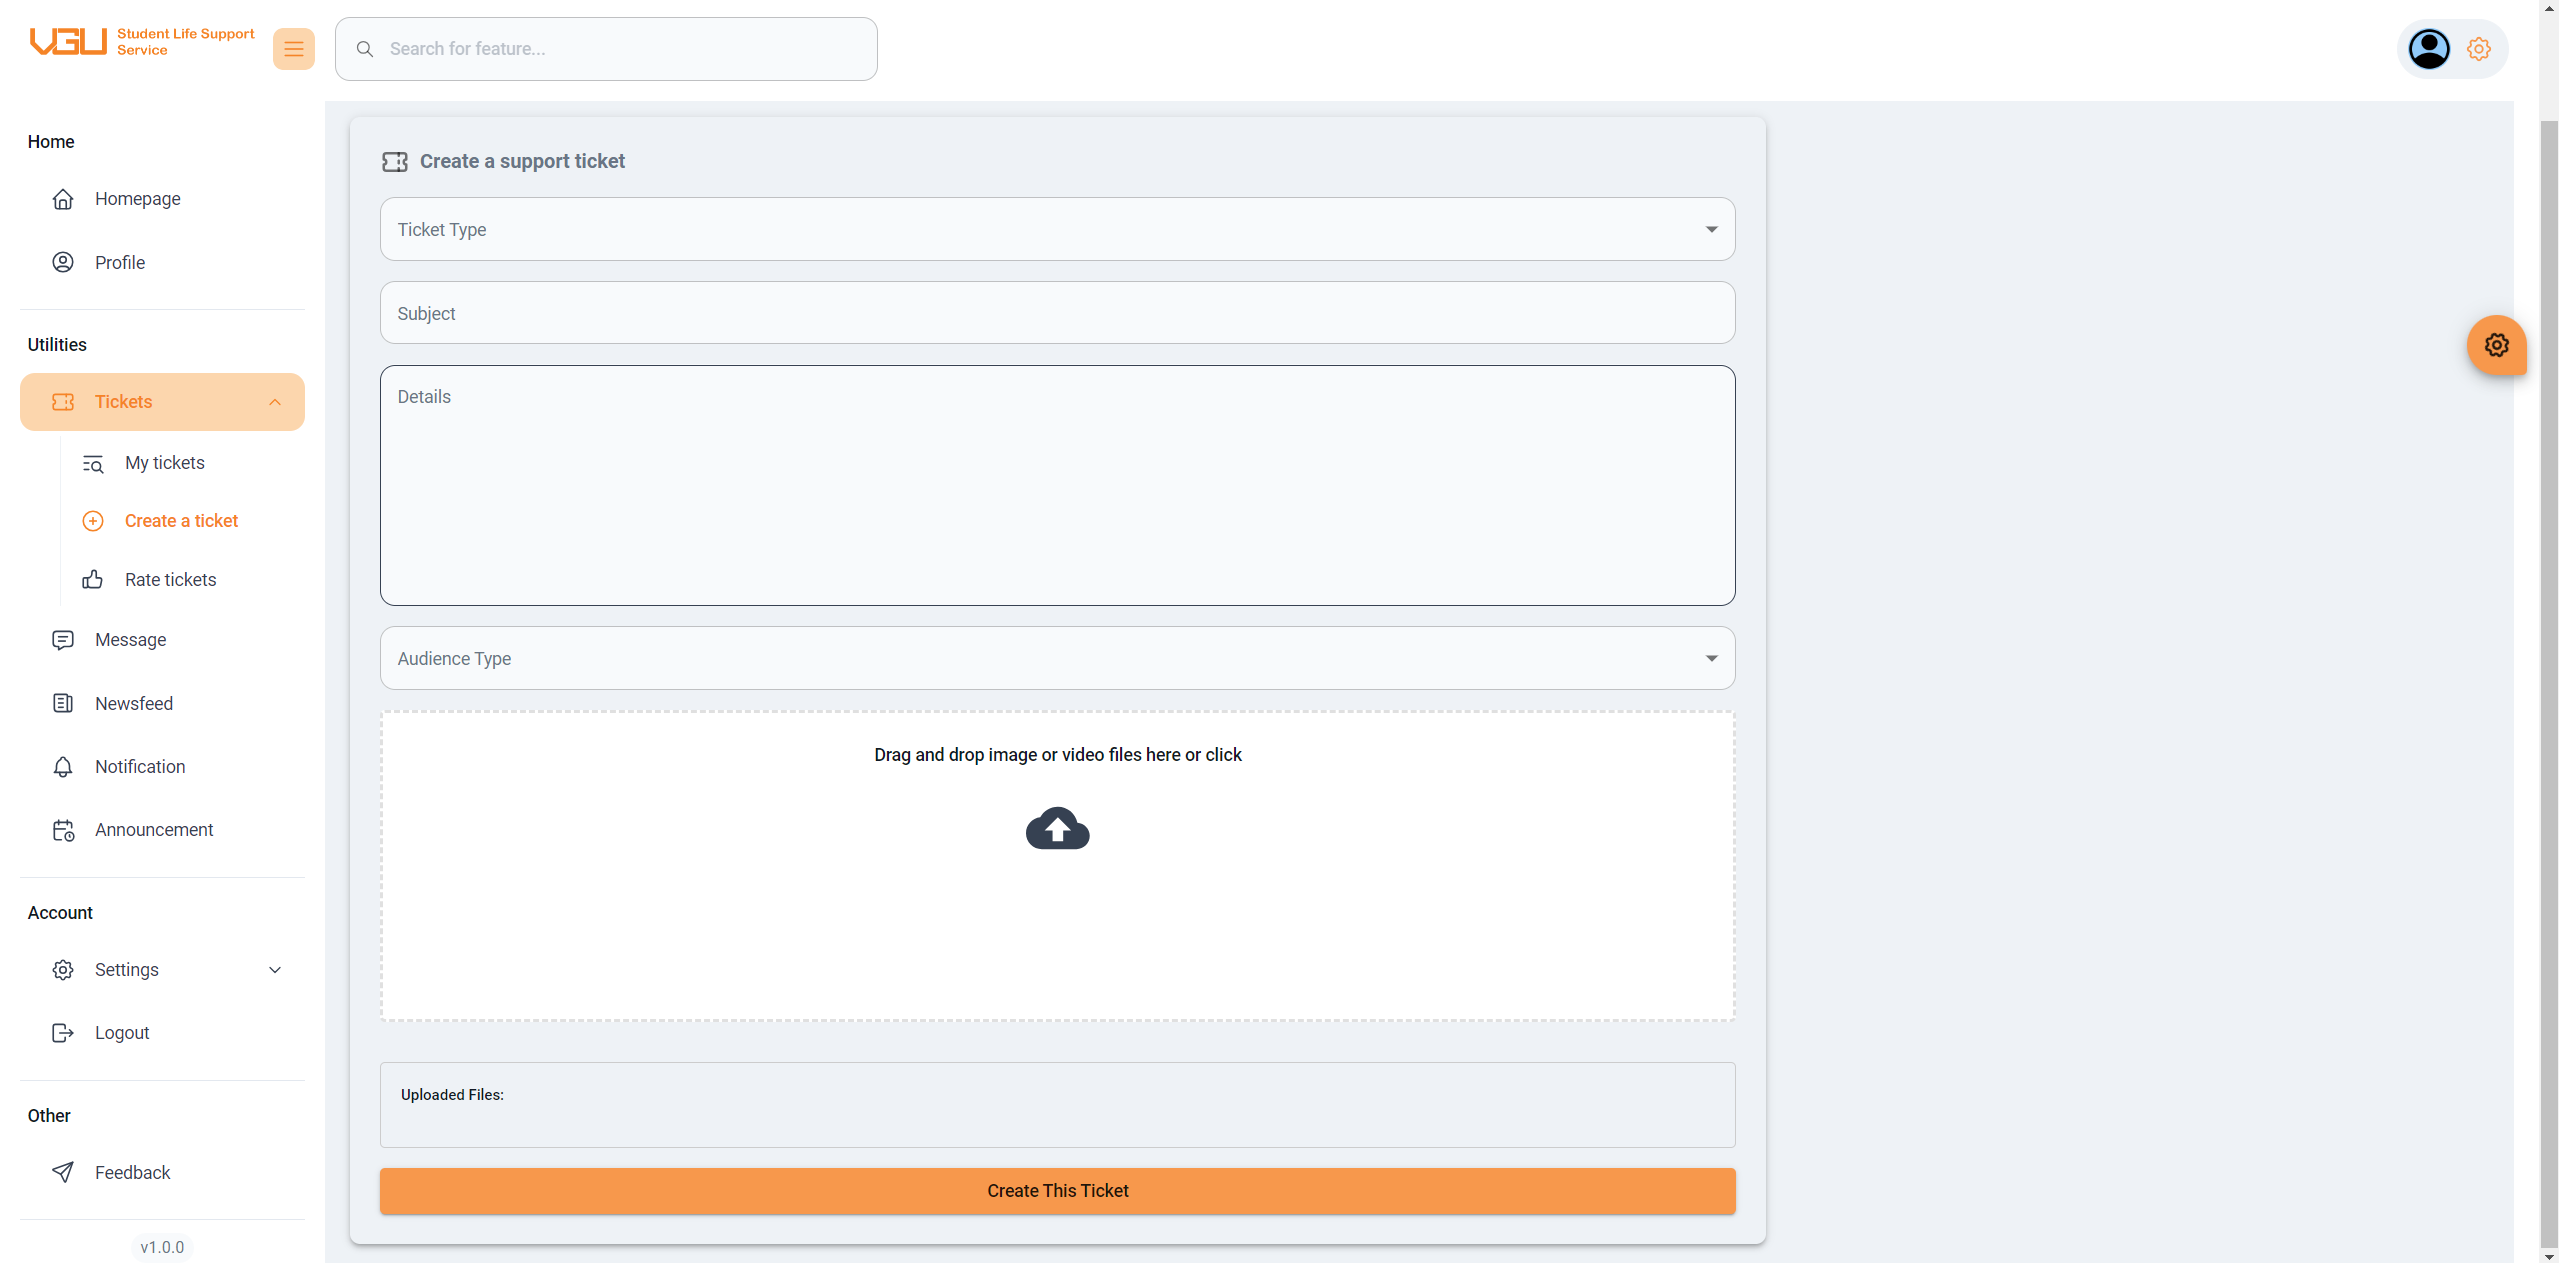
\includegraphics[width=1.0\linewidth]{graphics/gui/student/create-ticket}
		\caption{Student's Create Tickets Page}
		\label{fig:gui-std-create-ticket}
	\end{figure}
	
	
	\subsubsection{Rate Tickets}
	\begin{figure}[H]
		\centering
		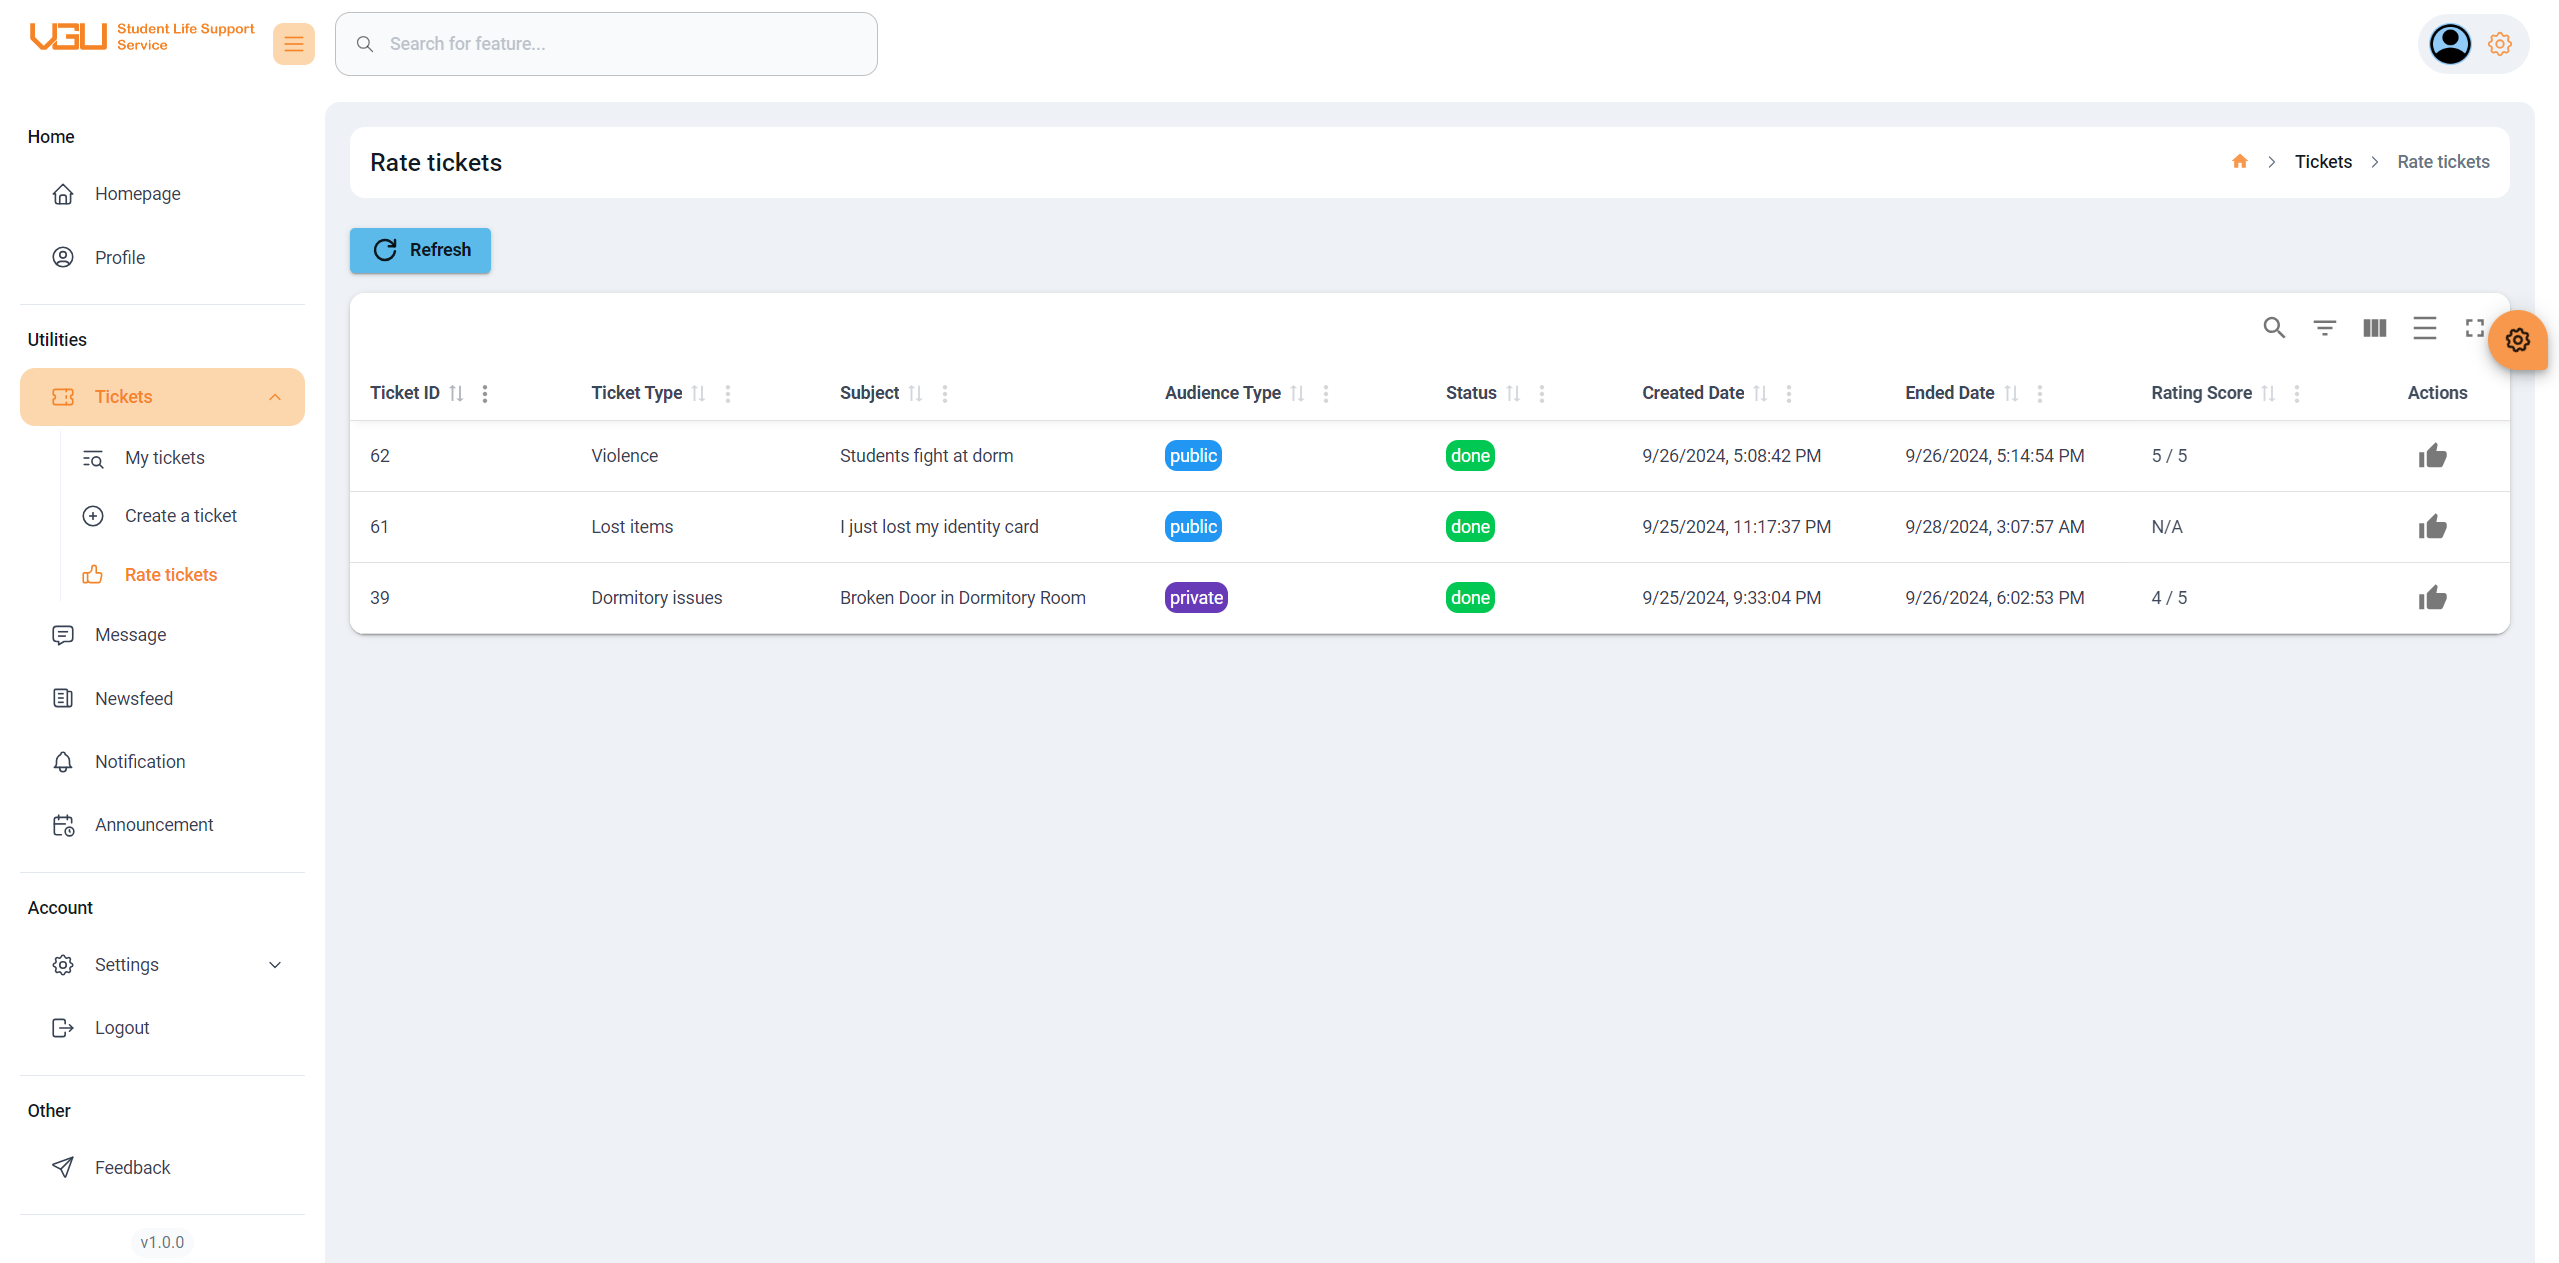
\includegraphics[width=1.0\linewidth]{graphics/gui/student/rate-ticket}
		\caption{Student's Rate Tickets Page}
		\label{fig:gui-std-rate-ticket}
	\end{figure}
	
	
	
	\begin{figure}[H]
		\centering
		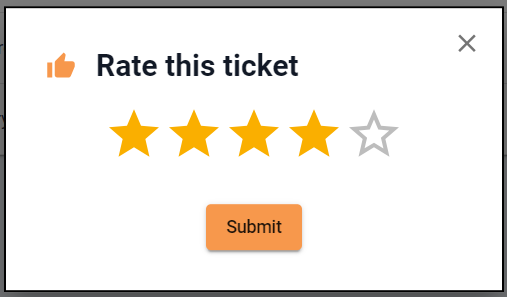
\includegraphics[width=0.5\linewidth]{graphics/gui/student/rate-ticket1}
		\caption{Submit a ticket rating}
		\label{fig:gui-rate-ticket-modal}
	\end{figure}
	
	
	
	\subsubsection{Message}
	\begin{figure}[H]
		\centering
		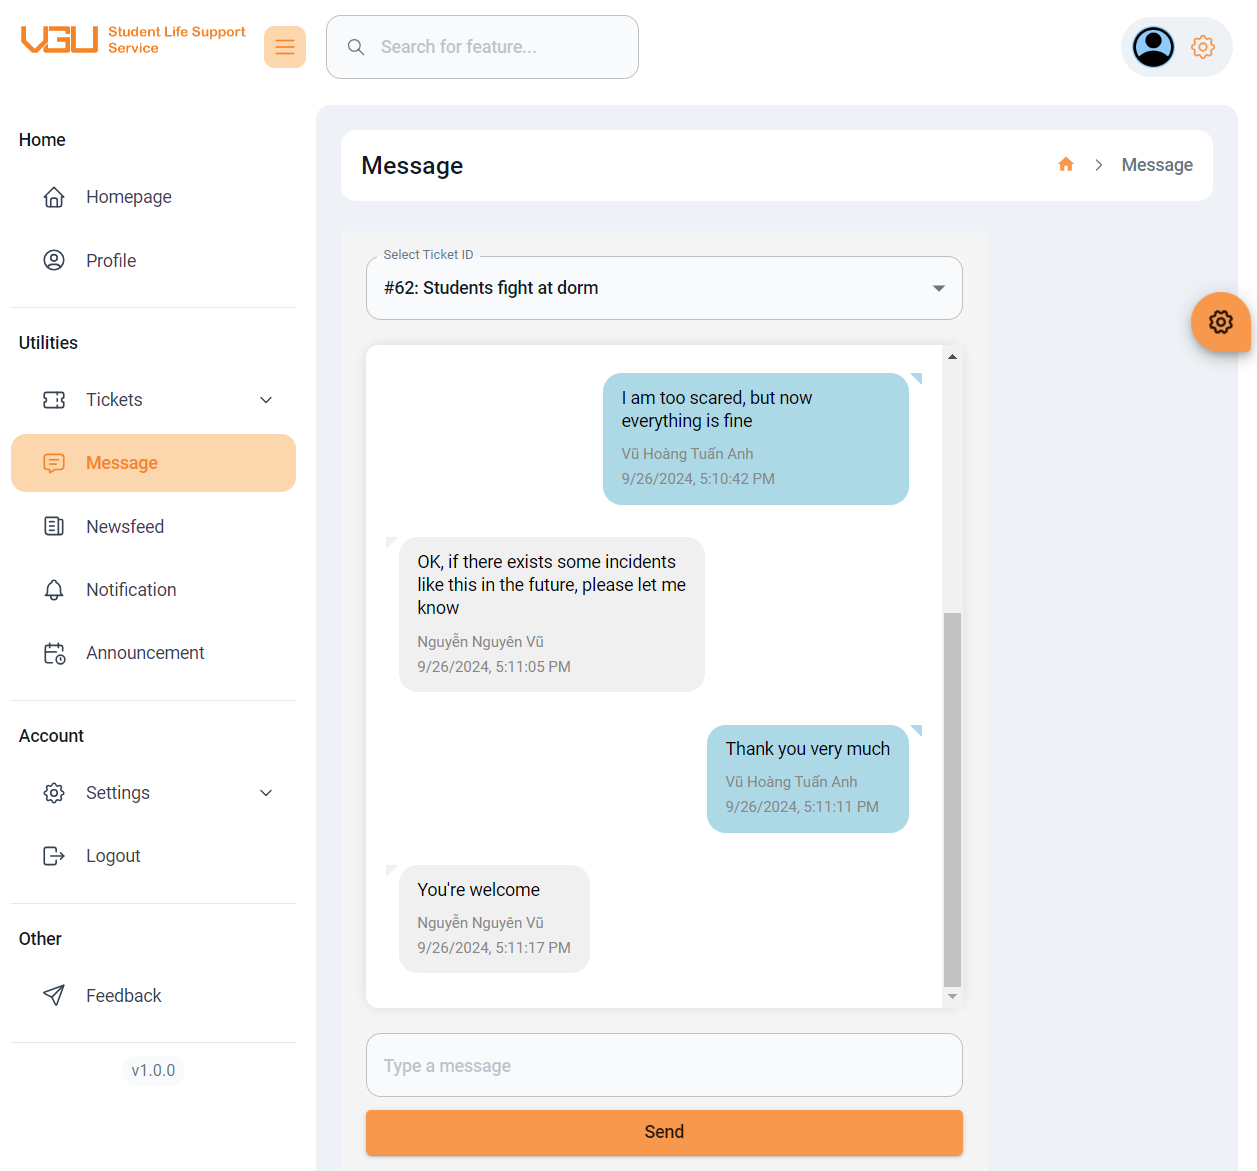
\includegraphics[width=1.0\linewidth]{graphics/gui/student/msg}
		\caption{Student's Message Page}
		\label{fig:msg}
	\end{figure}
	
	
	
	\subsubsection{Newsfeed}
	\begin{figure}[H]
		\centering
		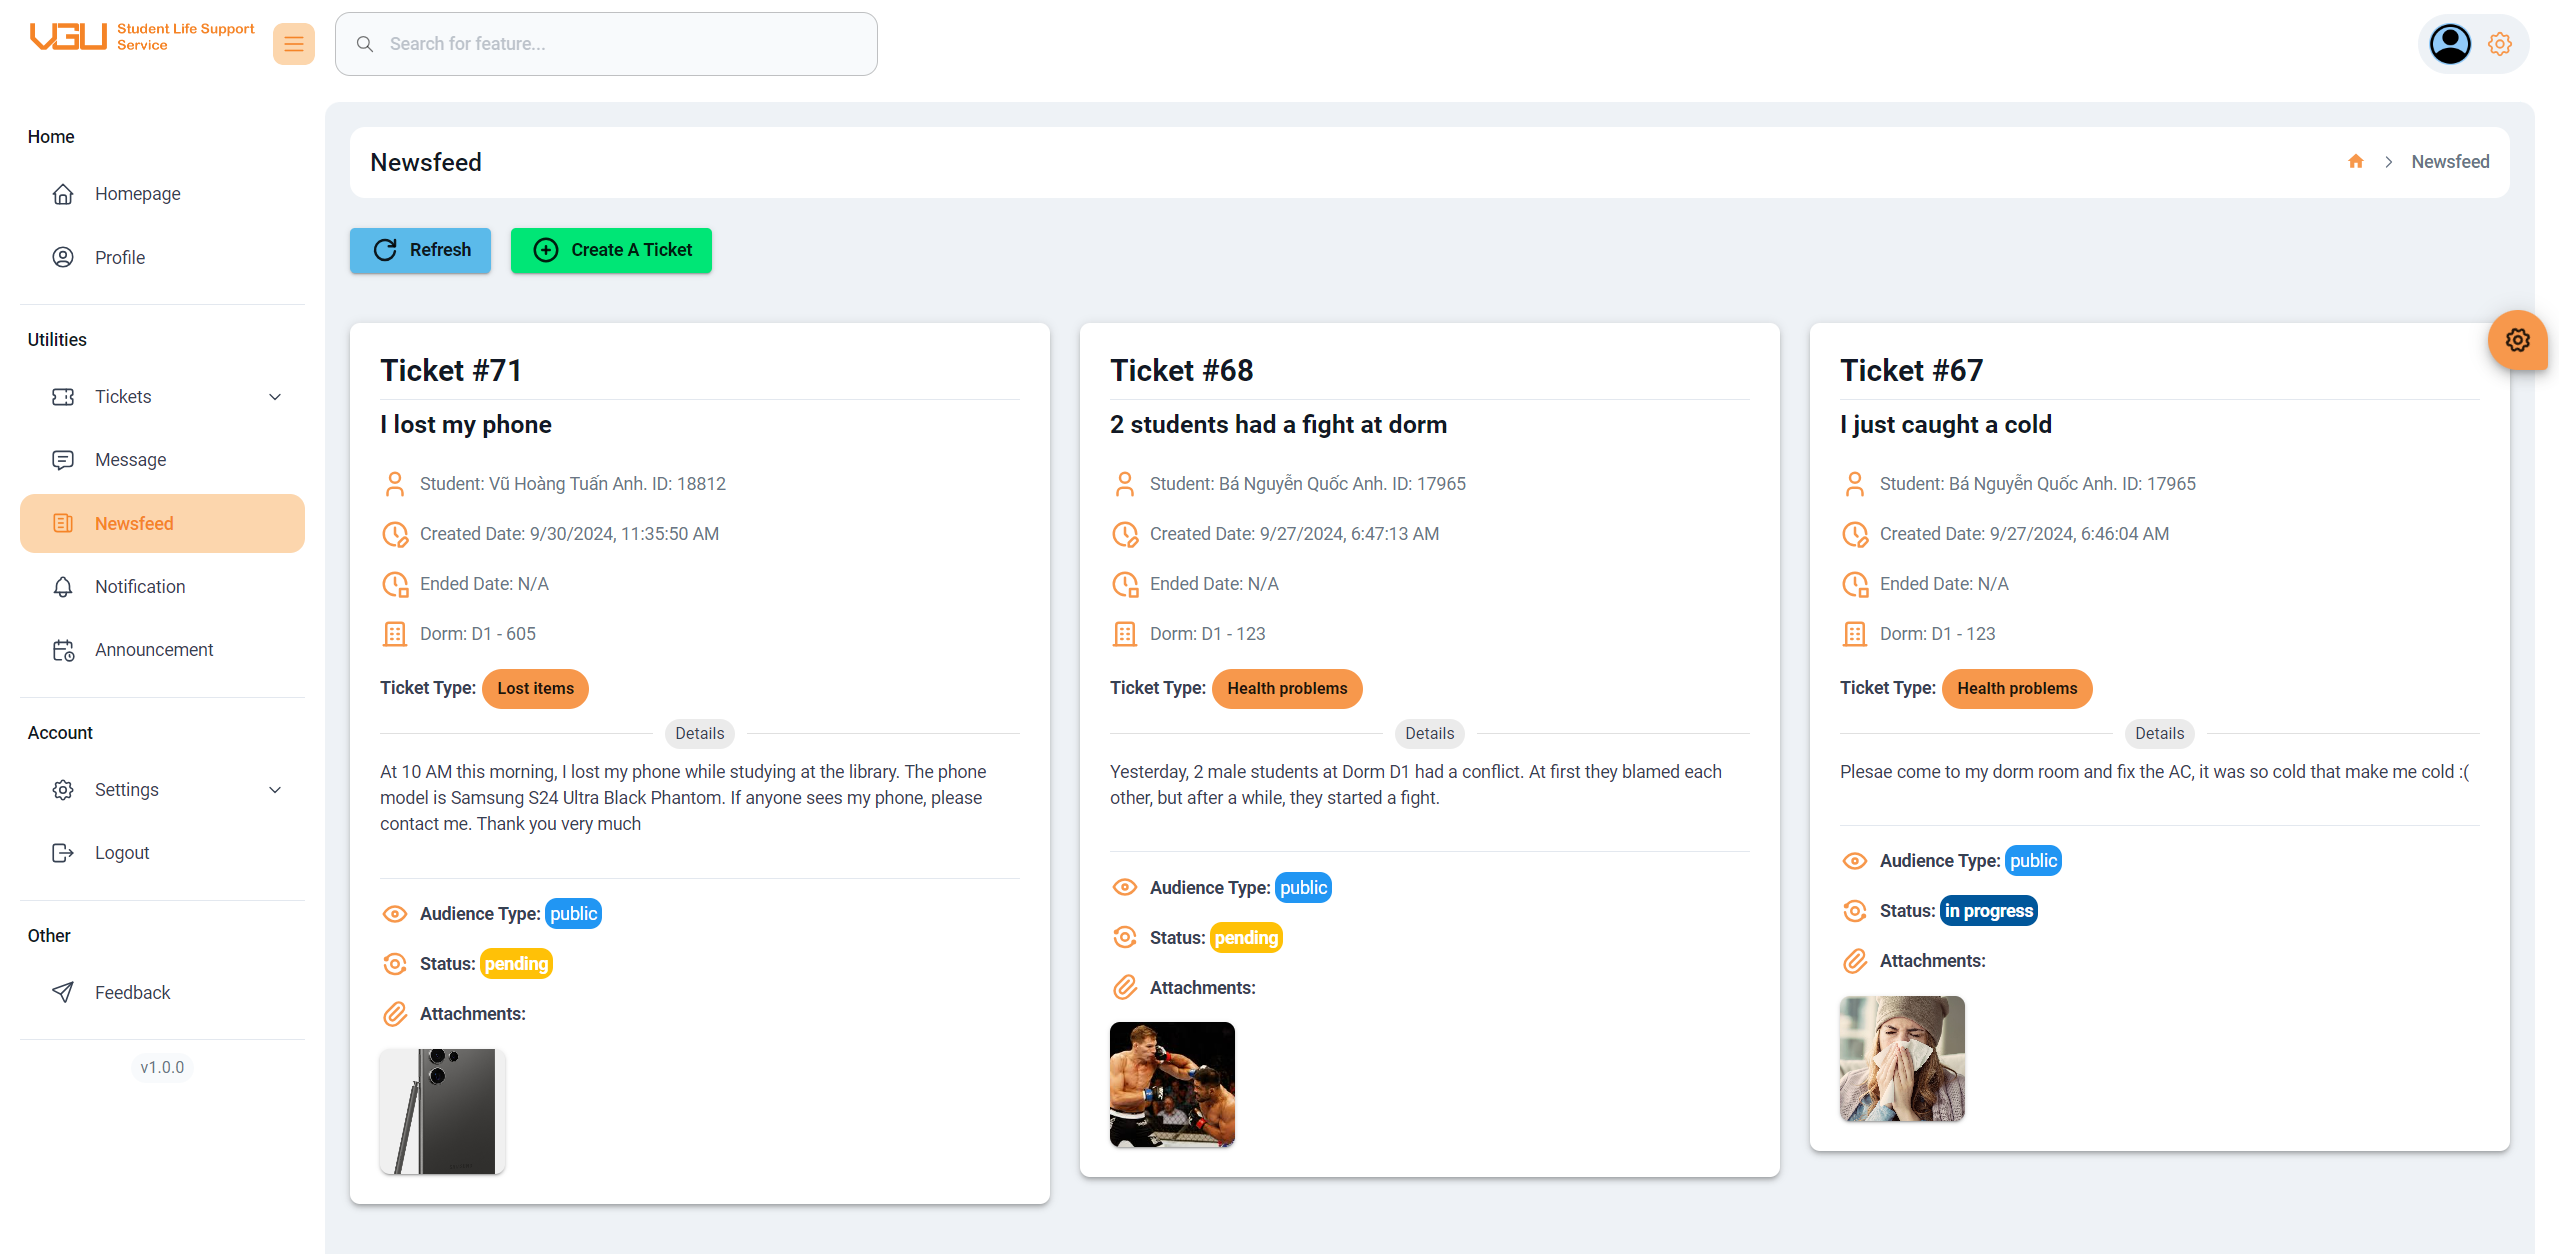
\includegraphics[width=1.0\linewidth]{graphics/gui/student/newsfeed}
		\caption{Student's Newsfeed}
		\label{fig:gui-std-newsfeed}
	\end{figure}
	
	
	
	\subsubsection{Notification}
	\begin{figure}[H]
		\centering
		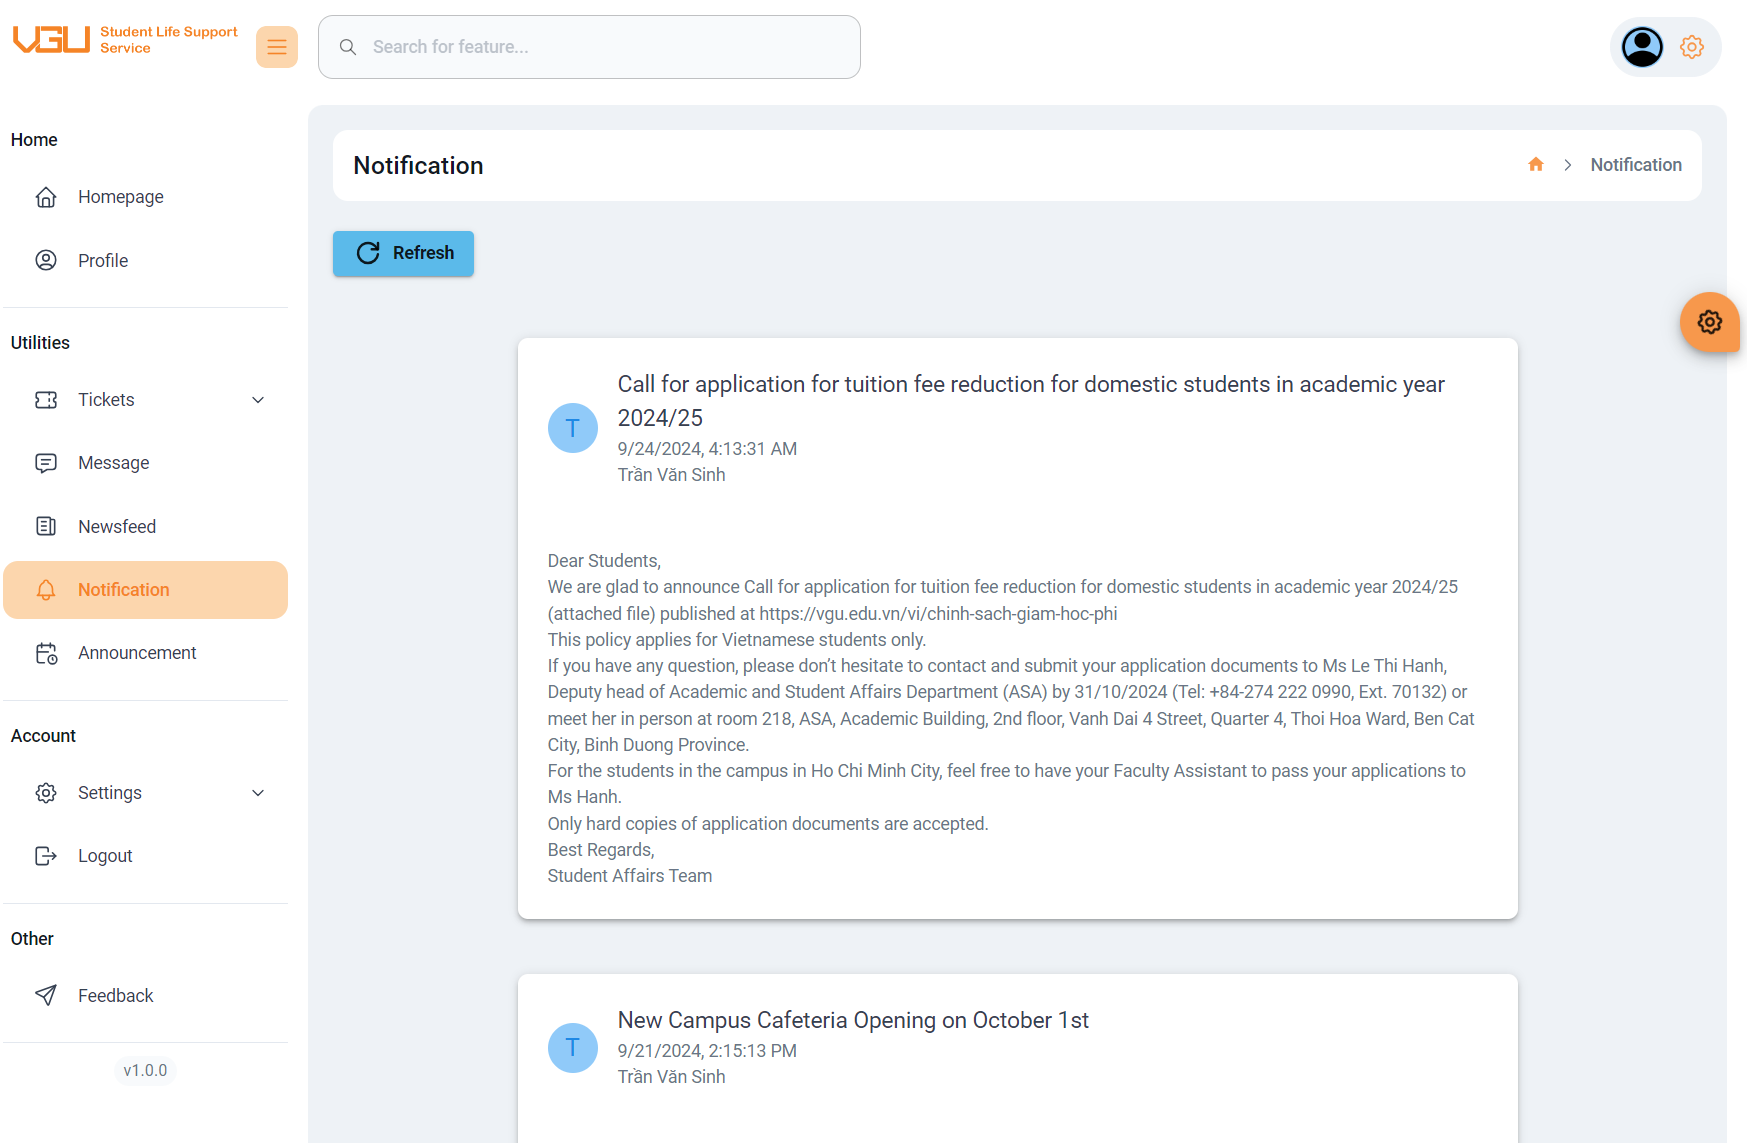
\includegraphics[width=1.0\linewidth]{graphics/gui/student/noti}
		\caption{Student's Notification Page}
		\label{fig:gui-std-noti}
	\end{figure}
	
	
	
	\subsubsection{Announcement}
	\begin{figure}[H]
		\centering
		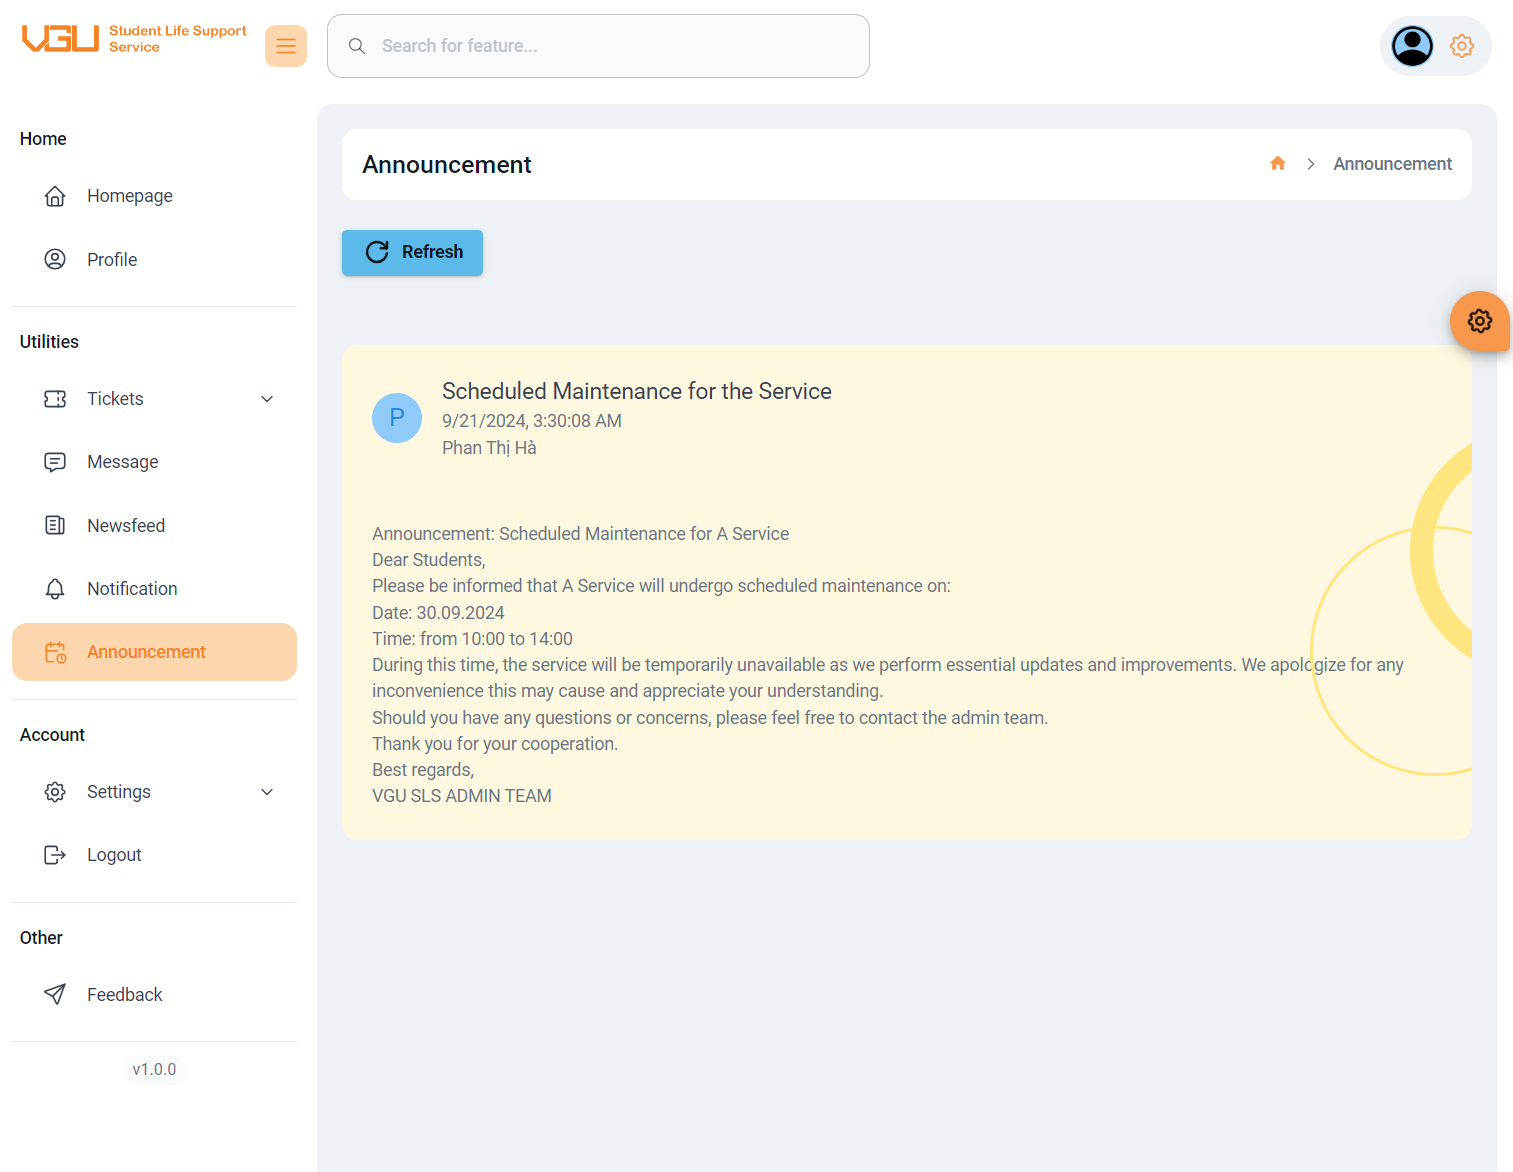
\includegraphics[width=1.0\linewidth]{graphics/gui/student/announcement}
		\caption{Student's Announcement Page}
		\label{fig:gui-std-announcement}
	\end{figure}
	
	
	\subsubsection{Settings}
	\begin{figure}[H]
		\centering
		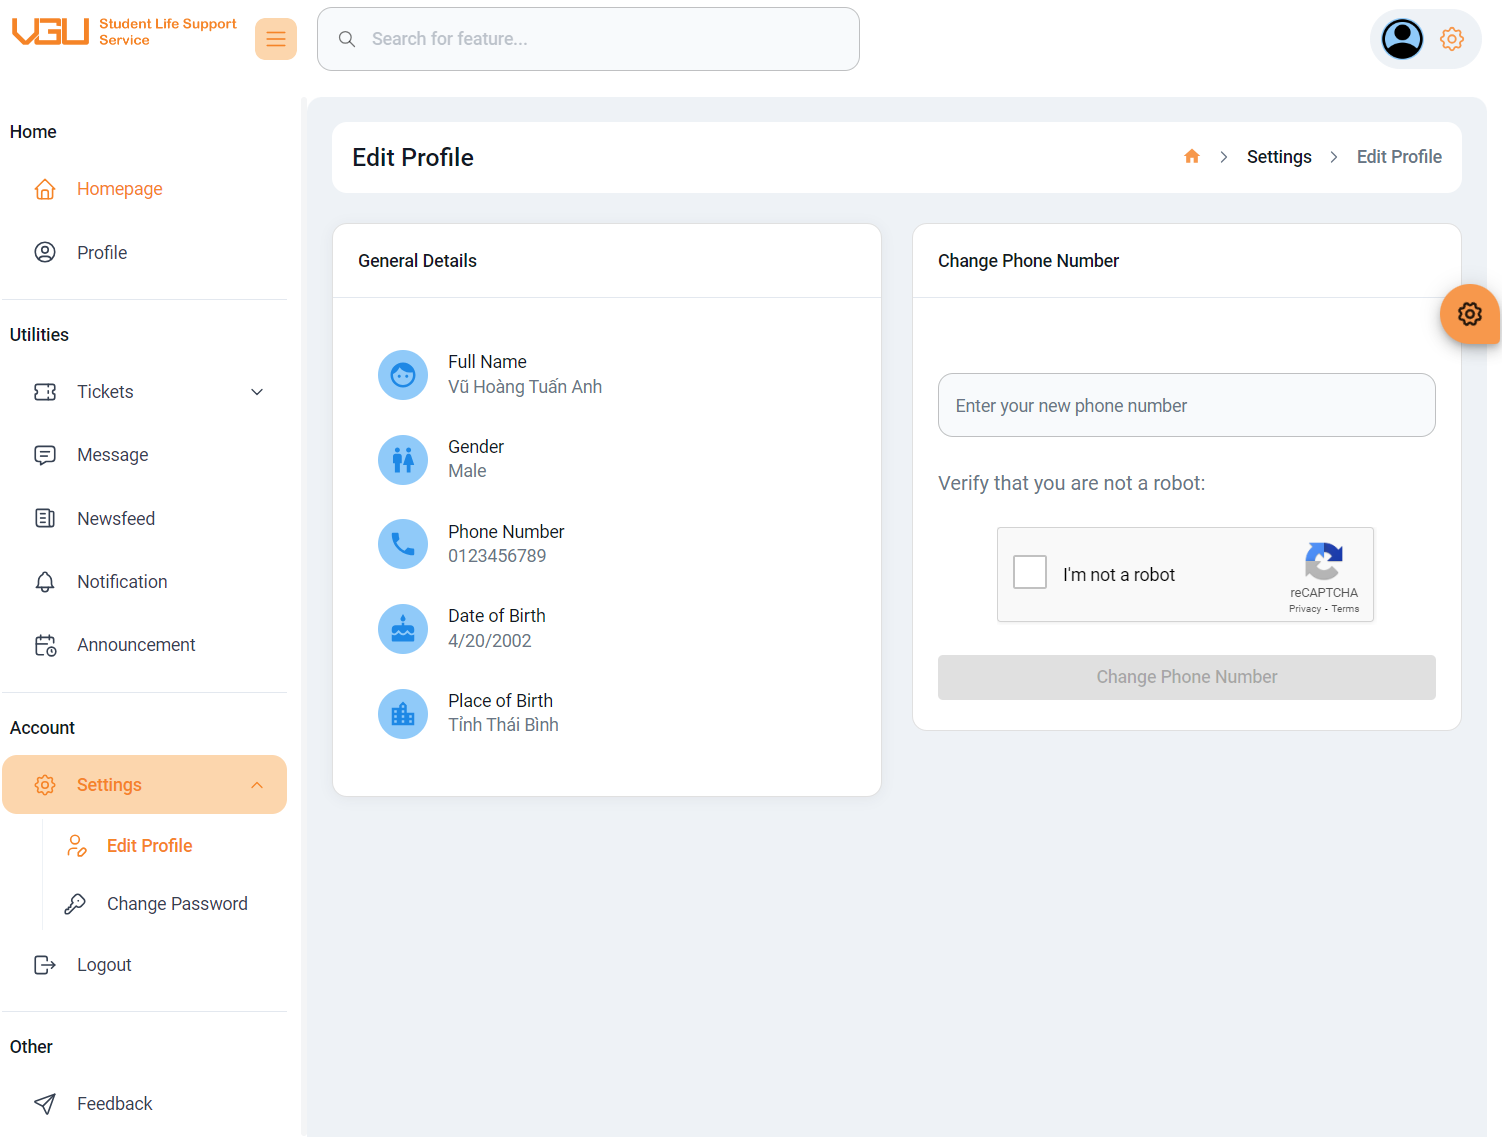
\includegraphics[width=1.0\linewidth]{graphics/gui/student/sett-edit-profile}
		\caption{Student's Edit Profile Page}
		\label{fig:gui-std-sett-edit-profile}
	\end{figure}
	
	
	\begin{figure}[H]
		\centering
		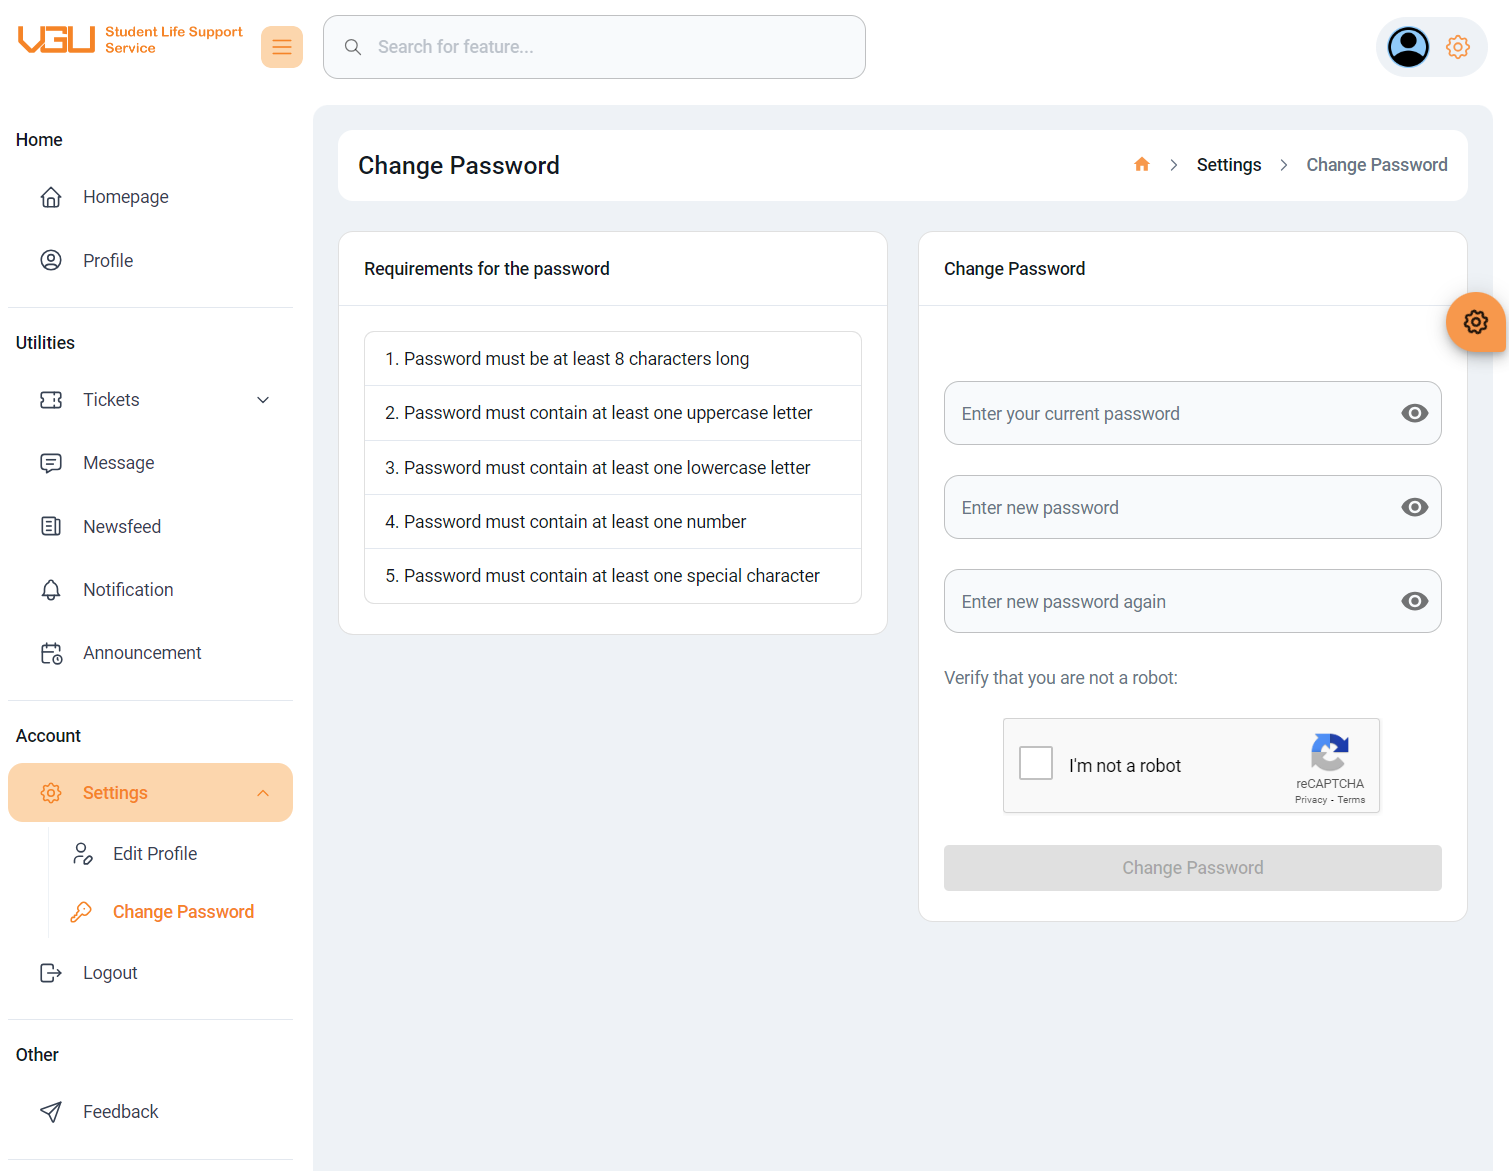
\includegraphics[width=1.0\linewidth]{graphics/gui/student/sett-password}
		\caption{Student's Change Password Page}
		\label{fig:gui-std-sett-password}
	\end{figure}
	
	
	\subsubsection{Feedback}
	\begin{figure}[H]
		\centering
		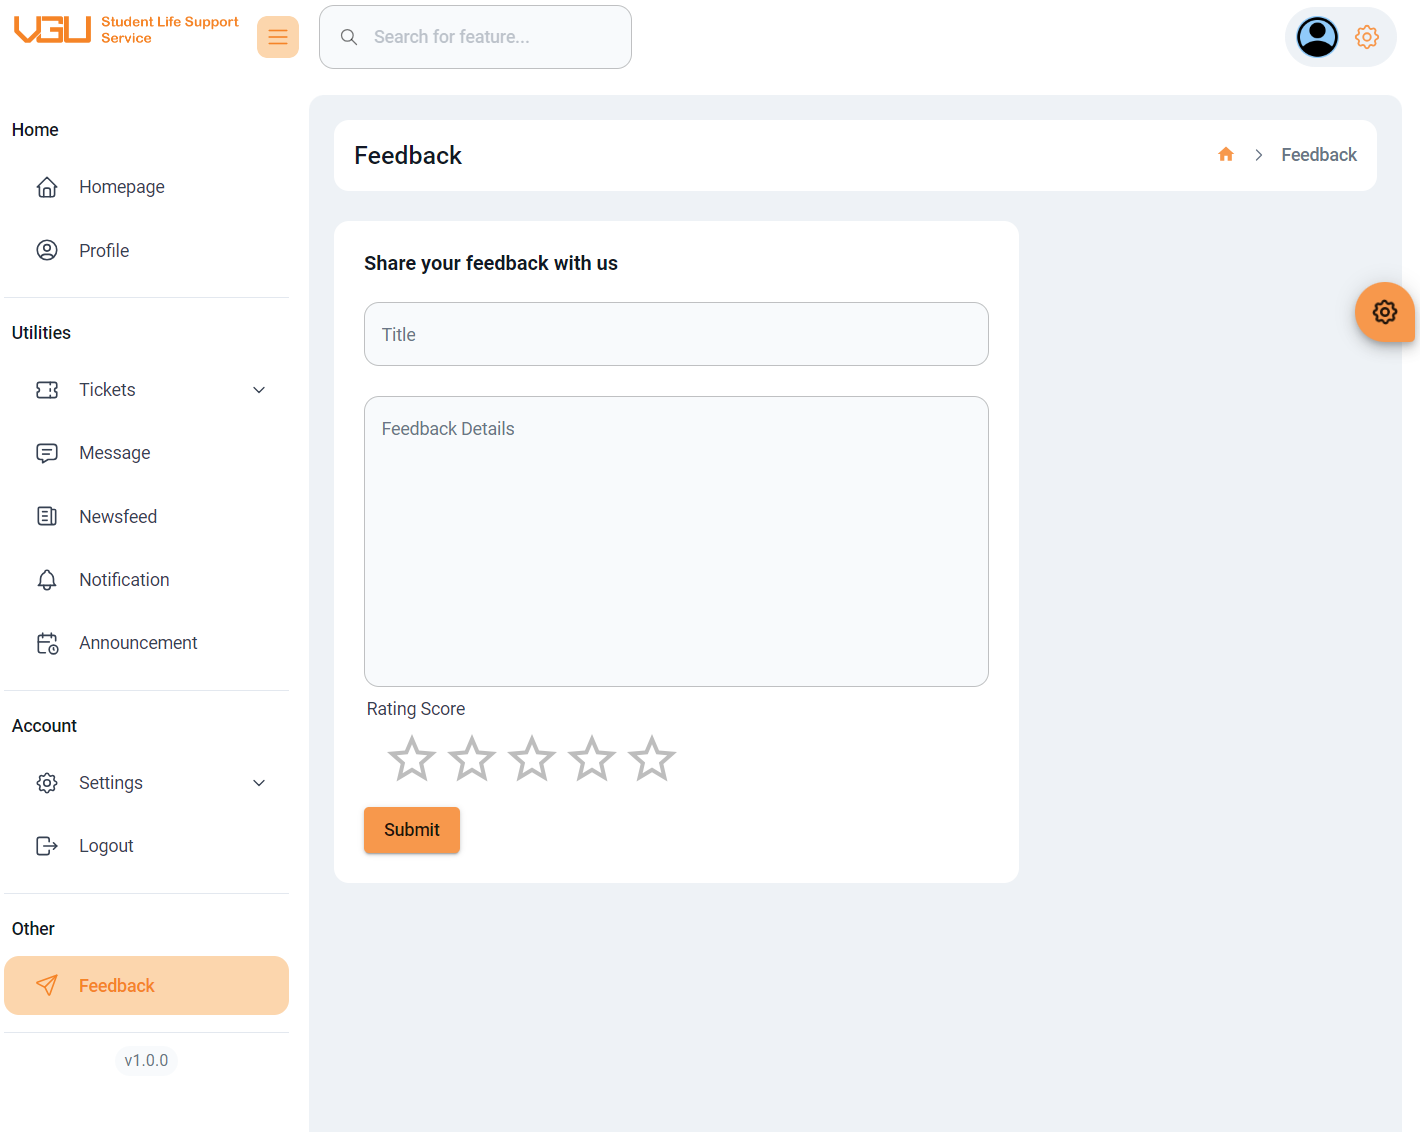
\includegraphics[width=1.0\linewidth]{graphics/gui/student/feedback}
		\caption{Student's Feedback Page}
		\label{fig:gui-std-feedback}
	\end{figure}
	
	
\subsection{Staff's functions}

	\subsubsection{Available Tickets}
	
	
	
	

	
	
	
	
	
	
	
	
	
	



